\chapter{初段ミューオントリガーシステム}
トリガーシステムの一つである初段ミューオントリガーシステムに着目し、本章では、Run-3におけるエンドキャプ部初段ミューオントリガーシステムについて述べる。

\section{ATLAS トリガーシステムの概要}
\subsubsection{Level1 Trigger}
・L1Calo\\
・L1Muon\\
\begin{figure}[tb]
  \centering
  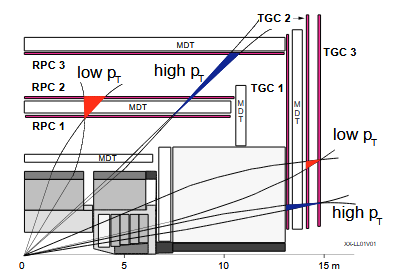
\includegraphics[clip, width=10cm]{fig/3/muon_trigger_overview.png}
  \caption{初段ミューオントリガー}
  \label{fig:muon}
\end{figure}

・Central Trigger
\subsubsection{High-Level Trigger}


\section{Run-3におけるエンドキャプ部初段ミューオントリガー}

\subsection{トリガーセクター}
ROIの話
\begin{figure}[tb]
  \centering
  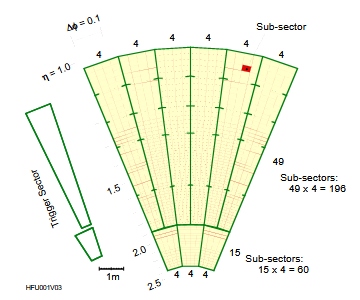
\includegraphics[clip, width=10cm]{fig/3/RoI.png}
  \caption{RoI}
  \label{fig:RoI}
\end{figure}


\subsection{ミューオンの運動量の算出}
運動量の算出の話
\begin{figure}[tb]
  \centering
  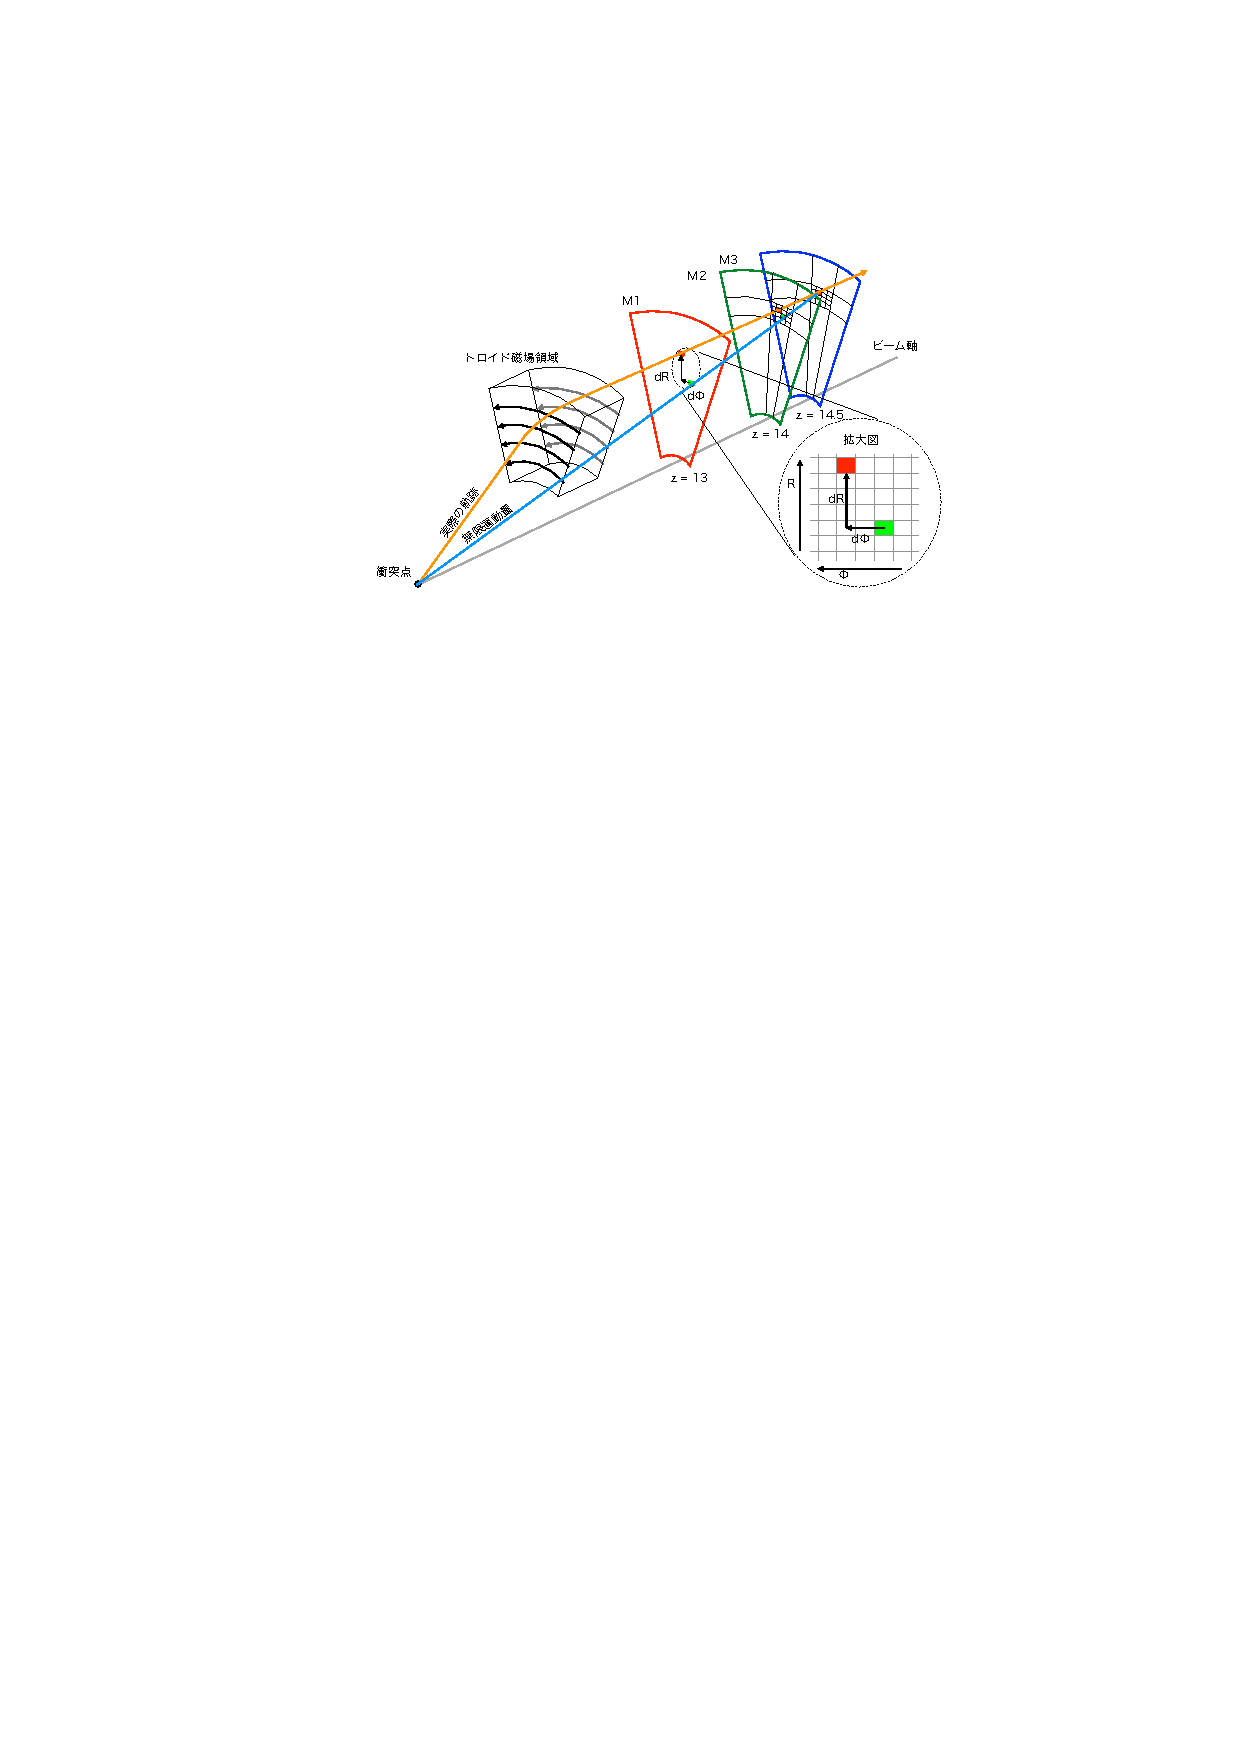
\includegraphics[clip, width=14cm]{fig/3/akatsuka_mt_trigger_scheme.pdf}
  \caption{ATLAS検出器エンドキャップ領域におけるトリガースキームの概念図\cite{article:akatsuka-mron}。無限大の運動量を持つミューオンを仮定し、磁場によって曲げられたミューオンとの位置の差を用いて$\pt$を計算する。}
  \label{fig:trigger-scheme}
\end{figure}

\subsubsection{Coincidence Window}
・CWの話
・現行CWの作成手法

\subsection{エレクトロニクス}

\section{Run-3初期における初段ミューオントリガーの性能}
・Efficiency
・Rate
問題点 電荷 位置

\section{本研究の目的}
・検出器のズレ<Run-2での検出器のズレの測定図>
\begin{figure}[tb]
  \centering
  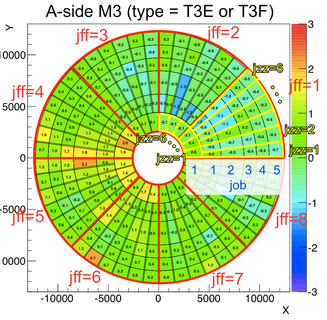
\includegraphics[clip, width=10cm]{fig/4/zure.png}
  \caption{Resolution}
  \label{fig:Resolution}
\end{figure}

\subsection{Run-2における最適化}
山内さん
・検出器アライメント
<木戸さんの手法の説明>
\subsection{本研究の方針}
Run-3における初段ミューオントリガーの性能を向上させるために、現状では上記で述べた最適化手法を行う必要がある。しかし、Run-2で行われていた最適化手法は、各CWごとに1マスずつ6段階の閾値を確認する手法のため膨大な作業量が必用である。

・作業量が膨大
・機械学習に注目














